%\documentclass[10pt,xcolor={dvipsnames},fleqn]{beamer}
\documentclass[handout,10pt,xcolor={dvipsnames},fleqn]{beamer}
\usepackage{isse}


\usepackage{apalike}
\usepackage[utf8]{inputenc}
\usepackage{pdfpages}
%\usepackage{ngerman}
\usepackage{stmaryrd,amsmath,amssymb}
\usepackage{color}
\usepackage{enumerate}
\usepackage[makeroom]{cancel}
\usepackage{mdframed}
\usepackage{xskak}
\usepackage{fancyvrb}
\usepackage{marvosym}
\setchessboard{
showmover=false}
\usepackage[noend]{algpseudocode}   % package for algorithms
\usepackage{algorithm}
\usepackage{tikz}

\usepackage[absolute,overlay]{textpos}

\usetikzlibrary{trees,calc,shapes,arrows,matrix,shadows,decorations.markings}
\usetikzlibrary{decorations.pathreplacing}
\usetikzlibrary{calc,shapes.callouts,shapes.arrows}
\usetikzlibrary{decorations.text}
\newcommand{\CustomCite}[1]{\color{issegrey} \textbf{#1}}
\tikzset{
   hierNode/.style={main node,text width=1.1em,text centered,inner sep=1pt},
   bStyle/.style={fill=forestgreen!35},
   cStyle/.style={fill=black!35},
   dStyle/.style={fill=thermicred!25},
   optboundaries/.style={
           state,
           rectangle,
           rounded corners,
           draw=black, thick,
           minimum height=4em,
           minimum width=7em,
           inner sep=2pt,
           text centered,
           dashed
           },
  trajectory/.style={issegrey,-},
  emph/.style={isseorange},
  trajectorynode/.style={fill=issegrey},
  hystate/.style={
           state,
           rectangle,
           rounded corners,
           draw=black, very thick,
           minimum height=1em,
           minimum width=2em,
           inner sep=1pt,
           text centered,
           },
 hystatel/.style={
 		   hystate, 
 		   inner sep=3pt
 }
}


\mdfdefinestyle{theoremstyle}{
linecolor=red,linewidth=2pt,
frametitlerule=true,
frametitlebackgroundcolor=gray!20,
innertopmargin=\topskip,
}
\definecolor{LRed}{rgb}{1,.8,.8}
\definecolor{MRed}{rgb}{1,.6,.6}
\definecolor{HRed}{rgb}{1,.2,.2}

\usepackage{listings}
\lstdefinelanguage{mzn}
{
	morekeywords={var,morph,pareto,lex,par,int,solve,not,search,satisfy,new,endif,maximize,params,instantiates,with,bool,in,type,PVS,PVSType,minimize,float,constraint,soft,sum,forall,exists,array,of,include,predicate,then,commit,post,set,function,if,else,repeat,next,ann,break},
	sensitive=false,
	morecomment=[l]{\%},
	morecomment=[s]{/*}{*/},
	morestring=[b]",
}


\definecolor{lightlightgray}{gray}{0.95}
\definecolor{forestgreen}{HTML}{009B55}
\definecolor{thermicred}{rgb}{0.82, 0.1, 0.26}
\lstset
{
	basicstyle=\ttfamily\small,
	commentstyle=\ttfamily\color{thermicred},
	stringstyle=\ttfamily\color{isseorange},
	keywordstyle=\ttfamily\color{blue},
	tabsize=2,
	showstringspaces=false,
	flexiblecolumns=true,
	captionpos=b,	
	backgroundcolor=\color{lightlightgray},
	frame=single,
	 xleftmargin=\parindent,
}

\lstset{language=mzn}
\interfootnotelinepenalty=10000

% ====== custom commands

\newcommand{\prosumer}[1]{\ensuremath{\mathtt{#1}}}
% Soft Constraint Example
\newcommand{\constraintName}[1]{\ensuremath{\mathtt{#1}}}
% Biogas Constraints
\newcommand{\biogas}{biogas}
\newcommand{\biogasShort}{bio}
\newcommand{\gasFull}{\ensuremath{\constraintName{gasFull}_\mathtt{\biogasShort}}}
\newcommand{\ecoSweet}{\ensuremath{\constraintName{ecoSweet}_\mathtt{\biogasShort}}}
\newcommand{\onOff}{\ensuremath{\constraintName{onOff}_\mathtt{\biogasShort}}}
% Thermal Plant Constraints
\newcommand{\thermal}{thermal}
\newcommand{\thermalShort}{therm}
\newcommand{\ecoOpt}{\ensuremath{\constraintName{ecoOpt}_\mathtt{\thermalShort}}}
\newcommand{\inertia}{\ensuremath{\constraintName{inertia}_\mathtt{\thermalShort}}}
\newcommand{\ecoGood}{\ensuremath{\constraintName{ecoGood}_\mathtt{\thermalShort}}}
\newcommand{\hLevelThermal}[1]{$H_#1^\mathtt{\thermalShort}$}
% Electric Vehicle
\newcommand{\ev}{EV}
\newcommand{\limitBatteryUsage}{\ensuremath{\constraintName{limitBU}_\mathtt{\ev}}}
\newcommand{\prefBatteryLevel}{\ensuremath{\constraintName{prefBL}_\mathtt{\ev}}}
\newcommand{\earlyBird}{\ensuremath{\constraintName{earlyBird}_\mathtt{\ev}}}
% Organization
\newcommand{\org}{org}
\newcommand{\minMaxViolation}{\ensuremath{\constraintName{violation}_\mathtt{\org}}}
\newcommand{\hLevelOrg}[1]{$H_#1^\mathtt{\org}$}

\newcommand{\Variable}{X}
\newcommand{\LocalVariable}{\widehat{\Variable}}
\newcommand{\Domain}{D}
\newcommand{\Constraint}{C}
\newcommand{\ConstraintRelationship}{\mathcal{R}}

\newcommand{\valuation}{v}
\newcommand{\constraint}[1]{\mathrm{#1}}

\newcommand{\plantconstraint}[3]{  
\ifx#1b \constraint{best}[#3]
\else \ifx#1g \constraint{good}[#3]
\else \ifx#1a \constraint{acc}[#3]
\else \ifx#1d \constraint{diff}
\else \ifx#1l \constraint{low}[#3]
\else \ifx#1h \constraint{high}[#3]
\else \ifx#1o \constraint{org}[#3]
   \else
   \constraint{#1}_{#2}^{#3} 
   
   
\fi \fi \fi \fi \fi \fi \fi}
\usepackage{stmaryrd}

\providecommand{\smyth}[1]{\prec^{#1}}
\providecommand{\smytheq}[1]{\preceq^{#1}}

\providecommand{\checkfull}{\color{ForestGreen} \checkmark}
\providecommand{\checkhalf}{\color{BurntOrange} (\checkmark)}
\providecommand{\checknot}{\color{BrickRed} $x$}
% booktabs, tables 
\usepackage{booktabs}
\usepackage{tabularx}
\usepackage{longtable}
\usepackage{dcolumn}
\newcolumntype{R}{>{\raggedleft\arraybackslash}X}
\newcolumntype{d}[1]{D{.}{.}{#1} }
\newcolumntype{L}[1]{>{\raggedright\let\newline\\\arraybackslash\hspace{0pt}}m{#1}}


\newcommand{\RN}[1]{%
  \textup{\uppercase\expandafter{\romannumeral#1}}%
}

\newcommand{\code}[1]{\normalfont\texttt{\spaceskip=3pt\frenchspacing\def\{{\char123}\def\}{\char125}\def\^{\char94}\def\_{\char95}#1}}
\newcommand{\varit}[1]{{\frenchspacing\ensuremath{\normalfont\textsl{#1}}}}
\newcommand{\macit}[1]{{\frenchspacing\ensuremath{\normalfont\textsf{#1}}}}
\newcommand{\Eta}{\mathrm{H}}
\newcommand{\Mu}{\mathrm{M}}
\newcommand{\Nu}{\mathrm{N}}

\newcommand{\NZ}{\mathbb{N}}
\newcommand{\RZ}{\mathbb{R}}
\newcommand{\RZp}{\RZ_{\geq 0}}
\newcommand{\powerset}{\mathcal{P}}
\newcommand{\limp}{\mathrel{\Rightarrow}}
\newcommand{\compfun}{\mathbin{\circ}}
\newcommand{\isorel}{\mathrel{\cong}}
\newcommand{\restrict}[2]{{#1}\mathnormal{\upharpoonright}{#2}}
\newcommand{\natto}{\mathrel{\dot{\mathnormal{\to}}}}
\let\lbagold\lbag
\let\rbagold\rbag
\def\lbag{\mathopen{\lbagold}}
\def\rbag{\mathclose{\rbagold}}

\DeclareMathOperator{\Minop}{\mathrm{Min}}
\newcommand{\Min}[1]{\Minop^{#1}}
\DeclareMathOperator{\Maxop}{\mathrm{Max}}
\newcommand{\Max}[1]{\Maxop^{#1}}
\DeclareMathOperator{\finsets}{\mathcal{P}_{\mathrm{fin}}}
\DeclareMathOperator{\nefinsets}{\mathcal{P}_{\mathrm{fin}^+}}
%\DeclareMathOperator{\incfinsets}{\mathcal{I}_{\mathrm{fin}}}
\newcommand{\incfinsets}[1]{\mathcal{I}_{\mathrm{fin}}^{#1}}
\newcommand{\lowersubseteq}[1]{\mathrel{\subseteq_{#1}}}
\newcommand{\lowersupseteq}[1]{\mathrel{\supseteq_{#1}}}
\newcommand{\lowersubset}[1]{\mathrel{\subset_{#1}}}
\newcommand{\lowersupset}[1]{\mathrel{\supset_{#1}}}
\newcommand{\uppersubseteq}[1]{\mathrel{\subseteq^{#1}}}
\newcommand{\uppersupseteq}[1]{\mathrel{\supseteq^{#1}}}
\newcommand{\uppersubset}[1]{\mathrel{\subset^{#1}}}
\newcommand{\uppersupset}[1]{\mathrel{\supset^{#1}}}
\newcommand{\lowercup}[1]{\mathbin{\cup_{#1}}}
\newcommand{\uppercup}[1]{\mathbin{\cup^{#1}}}

\DeclareMathOperator{\finmsets}{\mathcal{M}_{\mathrm{fin}}}
\DeclareMathOperator{\nefinmsets}{\mathcal{M}_{\mathrm{fin}^+}}
\newcommand{\mcup}{\mathbin{\mathnormal{\cup}\llap{\text{\fontsize{8pt}{8pt}\selectfont$-$}}}}
\newcommand{\submseteq}{%
\mathrel{\mathchoice%
{\mathnormal{\subseteq}\llap{\text{\raisebox{0.3pt}{\fontsize{8pt}{8pt}\selectfont\rotatebox{90}{$-$}\hspace{1.8pt}}}}}%
{\mathnormal{\subseteq}\llap{\text{\raisebox{0.3pt}{\fontsize{8pt}{8pt}\selectfont\rotatebox{90}{$-$}\hspace{1.8pt}}}}}%
{\mathnormal{\subseteq}\llap{\text{\raisebox{-0.3pt}{\fontsize{5pt}{5pt}\selectfont\rotatebox{90}{$-$}\hspace{1.4pt}}}}}%
{\mathnormal{\subseteq}\llap{\text{\raisebox{-0.3pt}{\fontsize{5pt}{5pt}\selectfont\rotatebox{90}{$-$}\hspace{1.4pt}}}}}%
}}
\newcommand{\supmseteq}{\mathrel{\reflectbox{$\submseteq$}}}
\newcommand{\lowersubmseteq}[1]{\mathrel{\submseteq_{#1}}}
\newcommand{\uppersubmseteq}[1]{\mathrel{\submseteq^{#1}}}
\newcommand{\submset}{%
\mathrel{\mathchoice%
{\mathnormal{\subset}\llap{\text{\raisebox{-0.8pt}{\fontsize{8pt}{8pt}\selectfont\rotatebox{90}{$-$}\hspace{1.8pt}}}}}%
{\mathnormal{\subset}\llap{\text{\raisebox{-0.8pt}{\fontsize{8pt}{8pt}\selectfont\rotatebox{90}{$-$}\hspace{1.8pt}}}}}%
{\mathnormal{\subset}\llap{\text{\raisebox{-0.3pt}{\fontsize{7pt}{7pt}\selectfont\rotatebox{90}{$-$}\hspace{1pt}}}}}%
{\mathnormal{\subset}\llap{\text{\raisebox{-0.3pt}{\fontsize{7pt}{7pt}\selectfont\rotatebox{90}{$-$}\hspace{1pt}}}}}%
}}
\newcommand{\supmset}{\mathrel{\reflectbox{$\submset$}}}
\newcommand{\lowersubmset}[1]{\mathrel{\submset_{#1}}}
\newcommand{\uppersubmset}[1]{\mathrel{\submset^{#1}}}

\DeclareMathOperator{\collapseset}{\mathcal{C}}

\newcommand{\category}[1]{\mathrm{#1}}
\newcommand{\POcat}{\category{PO}}
\newcommand{\uSLcat}{\category{uSL}}
\newcommand{\poMoncat}{\category{poMon}}
\newcommand{\jMoncat}{\category{jMon}}
\newcommand{\mMoncat}{\category{mMon}}
\newcommand{\xMoncat}{{x}\category{Mon}}
\newcommand{\PVScat}{\category{PVS}}
\newcommand{\cSRngcat}{\category{cSRng}}
\newcommand{\DAGcat}{\category{DAG}}

\newcommand{\idfun}[1]{1_{#1}}
\newcommand{\functor}[1]{\mathit{#1}}
\DeclareMathOperator{\POfun}{\functor{PO}}
\DeclareMathOperator{\uSLfun}{\functor{uSL}}
\DeclareMathOperator{\poMonfun}{\functor{poMon}}
\DeclareMathOperator{\jMonfun}{\functor{jMon}}
\DeclareMathOperator{\mMonfun}{\functor{mMon}}
\DeclareMathOperator{\xMonfun}{\text{$x$}\functor{Mon}}
\DeclareMathOperator{\PVSfun}{\functor{PVS}}
\DeclareMathOperator{\cSRngfun}{\functor{cSRng}}
\DeclareMathOperator{\DAGfun}{\functor{DAG}}

\newcommand{\uSLfree}[1]{\uSLfun\langle#1\rangle}
\newcommand{\uSLeta}{\eta^{\uSLcat}}
\newcommand{\uSLetaat}[1]{\uSLeta_{#1}}
\newcommand{\uSLlift}[1]{{#1}^{\sharp_{\uSLcat}}}

\newcommand{\poMonfree}[1]{\poMonfun\langle#1\rangle}
\newcommand{\poMoneta}{\eta^{\poMoncat}}
\newcommand{\poMonetaat}[1]{\poMoneta_{#1}}
\newcommand{\poMonlift}[1]{{#1}^{\sharp_{\poMoncat}}}

\newcommand{\jMonfree}[1]{\jMonfun\langle#1\rangle}
\newcommand{\jMoneta}{\eta^{\jMoncat}}
\newcommand{\jMonetaat}[1]{\jMoneta_{#1}}
\newcommand{\jMonlift}[1]{{#1}^{\sharp_{\jMoncat}}}

\newcommand{\mMonfree}[1]{\mMonfun\langle#1\rangle}
\newcommand{\mMoneta}{\eta^{\mMoncat}}
\newcommand{\mMonetaat}[1]{\mMoneta_{#1}}
\newcommand{\mMonlift}[1]{{#1}^{\sharp_{\mMoncat}}}

\newcommand{\PVSfree}[1]{\PVSfun\langle#1\rangle}
\newcommand{\PVSeta}{\eta^{\PVScat}}
\newcommand{\PVSetaat}[1]{\PVSeta_{#1}}
\newcommand{\PVSlift}[1]{{#1}^{\sharp_{\PVScat}}}

\newcommand{\xMonfree}[1]{\xMonfun\langle#1\rangle}
\newcommand{\xMoneta}{\eta^{\xMoncat}}
\newcommand{\xMonetaat}[1]{\xMoneta_{#1}}
\newcommand{\xMonlift}[1]{{#1}^{\sharp_{\xMoncat}}}

\newcommand{\cSRngfree}[1]{\cSRngfun\langle#1\rangle}
\newcommand{\cSRngeta}{\eta^{\cSRngcat}}
\newcommand{\cSRngetaat}[1]{\cSRngeta_{#1}}
\newcommand{\cSRnglift}[1]{{#1}^{\sharp_{\cSRngcat}}}

\newcommand{\POfree}[1]{\POfun\langle#1\rangle}
\newcommand{\POeta}{\eta^{\POcat}}
\newcommand{\POetaat}[1]{\POeta_{#1}}
\newcommand{\POlift}[1]{{#1}^{\sharp_{\POcat}}}

\newcommand{\mtimes}[1]{\mathbin{\tilde{\cdot}_{#1}}}
\newcommand{\mplus}[1]{\mathbin{\tilde{\cup}_{#1}}}
\newcommand{\ftimes}[1]{\mathbin{\tilde{\mcup}^{#1}}}
\newcommand{\fplus}[1]{\mathbin{\tilde{\cup}_{#1}}}

\DeclareMathOperator{\scope}{\mathrm{sc}}
\DeclareMathOperator{\defdom}{\mathrm{def}}

\newcommand{\reflclos}[1]{\mathrel{(#1)^=}}
\newcommand{\transclos}[2][+]{\mathrel{(#2)^{#1}}}
\newcommand{\refltransclos}[1]{\mathrel{(#1)^*}}

\newcommand{\XPDrel}[2][\pi]{\rightsquigarrow^{#1}_{#2}}
\newcommand{\XPDreleq}[2][\pi]{\rightsquigarrow^{#1, =}_{#2}}
\newcommand{\XPDord}[2][\pi]{<^{#1}_{#2}}
\newcommand{\XPDordeq}[2][\pi]{\geq^{#1}_{#2}}
\newcommand{\XPDleq}[2][\pi]{\leq^{#1}_{#2}}
\newcommand{\XPDgeq}[2][\pi]{\geq^{#1}_{#2}}
\newcommand{\XPDw}[2][\pi]{w^{#1}_{#2}}
\newcommand{\XPDW}[2][\pi]{W^{#1}_{#2}}
\newcommand{\XPDk}[2][\pi]{k^{#1}_{#2}}

\newcommand{\SPDrel}{\XPDrel[\mathrm{SPD}]}
\newcommand{\SPDreleq}{\XPDreleq[\mathrm{SPD}]}
\newcommand{\SPDleq}{\XPDleq[\mathrm{SPD}]}
\newcommand{\SPDgeq}{\XPDgeq[\mathrm{SPD}]}
\newcommand{\SPDord}{\XPDord[\mathrm{SPD}]}
\newcommand{\SPDw}{\XPDw[\mathrm{SPD}]}
\newcommand{\SPDW}{\XPDW[\mathrm{SPD}]}
\newcommand{\DPDrel}{\XPDrel[\mathrm{DPD}]}
\newcommand{\DPDreleq}{\XPDreleq[\mathrm{DPD}]}
\newcommand{\DPDord}{\XPDord[\mathrm{DPD}]}
\newcommand{\DPDw}{\XPDw[\mathrm{DPD}]}
\newcommand{\DPDW}{\XPDW[\mathrm{DPD}]}
\newcommand{\TPDrel}{\XPDrel[\mathrm{TPD}]}
\newcommand{\TPDreleq}{\XPDreleq[\mathrm{TPD}]}
\newcommand{\TPDleq}{\XPDleq[\mathrm{TPD}]}
\newcommand{\TPDgeq}{\XPDgeq[\mathrm{TPD}]}
\newcommand{\TPDord}{\XPDord[\mathrm{TPD}]}
\newcommand{\TPDw}{\XPDw[\mathrm{TPD}]}
\newcommand{\TPDW}{\XPDW[\mathrm{TPD}]}

\DeclareMathSymbol{\UPi}{\mathalpha}{operators}{"05}



\renewcommand{\submseteq}{%
\mathrel{\mathchoice%
{\mathnormal{\subseteq}\llap{\text{\raisebox{0.0pt}{\fontsize{7.5pt}{7.5pt}\selectfont\rotatebox{90}{$-$}\hspace{1.6pt}}}}}%
{\mathnormal{\subseteq}\llap{\text{\raisebox{0.0pt}{\fontsize{7.5pt}{7.5pt}\selectfont\rotatebox{90}{$-$}\hspace{1.6pt}}}}}%
{\mathnormal{\subseteq}\llap{\text{\raisebox{-0.3pt}{\fontsize{7pt}{7pt}\selectfont\rotatebox{90}{$-$}\hspace{1pt}}}}}%
{\mathnormal{\subseteq}\llap{\text{\raisebox{-0.3pt}{\fontsize{7pt}{7pt}\selectfont\rotatebox{90}{$-$}\hspace{1pt}}}}}%
}}


\tikzset{
   main node/.style={circle,fill=black!15,draw,font=\sffamily},
   constraint node/.style={main node, circle, inner sep=2pt,font=\sffamily\small},   
   treestyle/.style={rectangle,fill=black!15,draw,font=\sffamily}
}


\mdtheorem[style=theoremstyle]{definition}{Definition}

\renewcommand{\vec}[1]{\mathbf{#1}}
\newcommand{\tupleOf}[1]{\langle #1 \rangle}
\newcommand{\cemph}[1]{\alert{#1}}
\usepackage{framed}
\usepackage{ifthen}

\usetikzlibrary{decorations.pathmorphing,calc,shadows.blur,shadings}
\usetikzlibrary{mindmap,trees,automata,arrows}
\usepackage{extrabeamercmds}

\newcommand{\hFirst}[1]{{\color{isseorange} #1}}
\newcommand{\hSecond}[1]{{\color{CornflowerBlue} #1}}

\newcounter{mathseed}
\setcounter{mathseed}{3}
\pgfmathsetseed{\arabic{mathseed}} % To have predictable results
% Define a background layer, in which the parchment shape is drawn
\pgfdeclarelayer{background}
\pgfsetlayers{background,main}


% This is the base for the fractal decoration. It takes a random point between the start and end, and
% raises it a random amount, thus transforming a segment into two, connected at that raised point
% This decoration can be applied again to each one of the resulting segments and so on, in a similar
% way of a Koch snowflake.
\pgfdeclaredecoration{irregular fractal line}{init}
{
  \state{init}[width=\pgfdecoratedinputsegmentremainingdistance]
  {
    \pgfpathlineto{\pgfpoint{random*\pgfdecoratedinputsegmentremainingdistance}{(random*\pgfdecorationsegmentamplitude-0.02)*\pgfdecoratedinputsegmentremainingdistance}}
    \pgfpathlineto{\pgfpoint{\pgfdecoratedinputsegmentremainingdistance}{0pt}}
  }
}


% define some styles
\tikzset{
   paper/.style={draw=black!10, blur shadow, every shadow/.style={opacity=1, black}, 
                 lower left=black!10, upper left=black!5, upper right=white, lower right=black!5, fill=none},
   irregular cloudy border/.style={decoration={irregular fractal line, amplitude=0.2},
           decorate,
     },
   irregular spiky border/.style={decoration={irregular fractal line, amplitude=-0.2},
           decorate,
     },
   ragged border/.style={ decoration={random steps, segment length=7mm, amplitude=2mm},
           decorate,
   }
}

\tikzset{
  normal border/.style={orange!30!black!10, decorate, 
     decoration={random steps, segment length=2.5cm, amplitude=.7mm}},
  torn border/.style={orange!30!black!5, decorate, 
     decoration={random steps, segment length=.5cm, amplitude=1.7mm}}}


\def\tornpaper#1{%
\ifthenelse{\isodd{\value{mathseed}}}{%
\tikz{
  \node[inner sep=1em] (A) {#1};  % Draw the text of the node
  \begin{pgfonlayer}{background}  % Draw the shape behind
  \fill[paper] % recursively decorate the bottom border
     \pgfextra{\pgfmathsetseed{\arabic{mathseed}}\addtocounter{mathseed}{1}}%
      {decorate[irregular cloudy border]{decorate{decorate{decorate{decorate[ragged border]{
        (A.north west) -- (A.north east)
      }}}}}}
      -- (A.south east)
     \pgfextra{\pgfmathsetseed{\arabic{mathseed}}}%
      {decorate[irregular spiky border]{decorate{decorate{decorate{decorate[ragged border]{
      -- (A.south west)
      }}}}}}
      -- (A.north west);
  \end{pgfonlayer}}
}{%
\tikz{
  \node[inner sep=1em] (A) {#1};  % Draw the text of the node
  \begin{pgfonlayer}{background}  % Draw the shape behind
  \fill[paper] % recursively decorate the bottom border
     \pgfextra{\pgfmathsetseed{\arabic{mathseed}}\addtocounter{mathseed}{1}}%
      {decorate[irregular spiky border]{decorate{decorate{decorate{decorate[ragged border]{
        (A.north east) -- (A.north west)
      }}}}}}
      -- (A.south west)
     \pgfextra{\pgfmathsetseed{\arabic{mathseed}}}%
      {decorate[irregular cloudy border]{decorate{decorate{decorate{decorate[ragged border]{
      -- (A.south east)
      }}}}}}
      -- (A.north east);
  \end{pgfonlayer}}
}}


% Macro to draw the shape behind the text, when it fits completly in the
% page
\def\parchmentframe#1{
\tikz{
  \node[inner sep=2em] (A) {#1};  % Draw the text of the node
  \begin{pgfonlayer}{background}  % Draw the shape behind
  \fill[normal border] 
        (A.south east) -- (A.south west) -- 
        (A.north west) -- (A.north east) -- cycle;
  \end{pgfonlayer}}}

% Macro to draw the shape, when the text will continue in next page
\def\parchmentframetop#1{
\tikz{
  \node[inner sep=2em] (A) {#1};    % Draw the text of the node
  \begin{pgfonlayer}{background}    
  \fill[normal border]              % Draw the ``complete shape'' behind
        (A.south east) -- (A.south west) -- 
        (A.north west) -- (A.north east) -- cycle;
  \fill[torn border]                % Add the torn lower border
        ($(A.south east)-(0,.2)$) -- ($(A.south west)-(0,.2)$) -- 
        ($(A.south west)+(0,.2)$) -- ($(A.south east)+(0,.2)$) -- cycle;
  \end{pgfonlayer}}}

% Macro to draw the shape, when the text continues from previous page
\def\parchmentframebottom#1{
\tikz{
  \node[inner sep=2em] (A) {#1};   % Draw the text of the node
  \begin{pgfonlayer}{background}   
  \fill[normal border]             % Draw the ``complete shape'' behind
        (A.south east) -- (A.south west) -- 
        (A.north west) -- (A.north east) -- cycle;
  \fill[torn border]               % Add the torn upper border
        ($(A.north east)-(0,.2)$) -- ($(A.north west)-(0,.2)$) -- 
        ($(A.north west)+(0,.2)$) -- ($(A.north east)+(0,.2)$) -- cycle;
  \end{pgfonlayer}}}

% Macro to draw the shape, when both the text continues from previous page
% and it will continue in next page
\def\parchmentframemiddle#1{
\tikz{
  \node[inner sep=2em] (A) {#1};   % Draw the text of the node
  \begin{pgfonlayer}{background}   
  \fill[normal border]             % Draw the ``complete shape'' behind
        (A.south east) -- (A.south west) -- 
        (A.north west) -- (A.north east) -- cycle;
  \fill[torn border]               % Add the torn lower border
        ($(A.south east)-(0,.2)$) -- ($(A.south west)-(0,.2)$) -- 
        ($(A.south west)+(0,.2)$) -- ($(A.south east)+(0,.2)$) -- cycle;
  \fill[torn border]               % Add the torn upper border
        ($(A.north east)-(0,.2)$) -- ($(A.north west)-(0,.2)$) -- 
        ($(A.north west)+(0,.2)$) -- ($(A.north east)+(0,.2)$) -- cycle;
  \end{pgfonlayer}}}

% Define the environment which puts the frame
% In this case, the environment also accepts an argument with an optional
% title (which defaults to ``Example'', which is typeset in a box overlaid
% on the top border
\newenvironment{parchment}[1][Example]{%
  \def\FrameCommand{\parchmentframe}%
  \def\FirstFrameCommand{\parchmentframetop}%
  \def\LastFrameCommand{\parchmentframebottom}%
  \def\MidFrameCommand{\parchmentframemiddle}%
  \vskip\baselineskip
  \MakeFramed {\FrameRestore}
  \noindent\tikz\node[inner sep=1ex, draw=black!20,fill=white, 
          anchor=west, overlay] at (0em, 2em) {\sffamily#1};\par}%
{\endMakeFramed}


\title{MiniBrass: Soft Constraint Programming}
\author{Alexander Schiendorfer et al.}

\date{\today}

\begin{document}
\titleframe


\tikzset{
    process/.style={rectangle,rounded corners,draw=black, top color=isseorange!5, bottom color=isseorange!30},
    file/.style={rectangle,draw=black}
}



\begin{frame}[fragile]{Mentor Matching}

\textbf{Ziel}: Teile Mentees (z.B. Studenten) Mentoren zu (z.B. Firmen), sodass
\begin{itemize}
\item Studenten sind sehr zufrieden mit ihren Mentoren
\item Firmen sind mit ihren Mentees ebenfalls zufrieden
\item Zweiseitige Präferenzen
\end{itemize}

\vspace*{2ex}

Bisher klingt das wie ein typisches \emph{Stable Matching}-Problem, aber:

\begin{itemize}
\item Es gibt keine 1:1 Abbildung (Firmen betreuen mehrere Studenten)
\item Zusätzliche Constraints sind vorhanden:
\begin{itemize}
\item[-] Jede Firme betreut zumindest $l$, höchstens aber $u$ Studenten
\item[-] Die Anzahl betreuter Studenten \emph{sollten} ungefähr gleich sein pro Firma (Fairness)
\item[-] Studenten, die eine Firma ``verachten'', sollen nicht gezwungen werden (\emph{harter Ausschluss} von Lösungen)
\end{itemize}
\end{itemize}
\end{frame}


\begin{frame}[fragile]{Mentor Matching: Beispiel}
\begin{center}
\tikzset{onslide/.code args={<#1>#2}{%
  \only<#1>{\pgfkeysalso{#2}}
}}

\tikzstyle{highlight}=[isseorange,ultra thick]
\tikzstyle{highlight2}=[CornflowerBlue,ultra thick,rounded corners]
\tikzstyle{defaultStyle}=[white,ultra thick,rounded corners]

\tikzstyle{impo}=[dashed]
\begin{tikzpicture}[every node/.style={
anchor=base,
%text depth=.5ex,
%text height=2ex,
%minimum height=2ex,
align=center,
rectangle,
text width=2em
}]
\matrix (magic) [nodes in empty cells, ampersand replacement=\&,row sep=0.4cm,column sep=1.5cm]
{
\node[draw,defaultStyle, onslide={<3->{highlight2}}](s1){
\includegraphics[width=\textwidth]{img/businessman.png}}; \& \& \& \node[text width=4em, defaultStyle, draw, onslide={<3->{highlight2}}](c1) {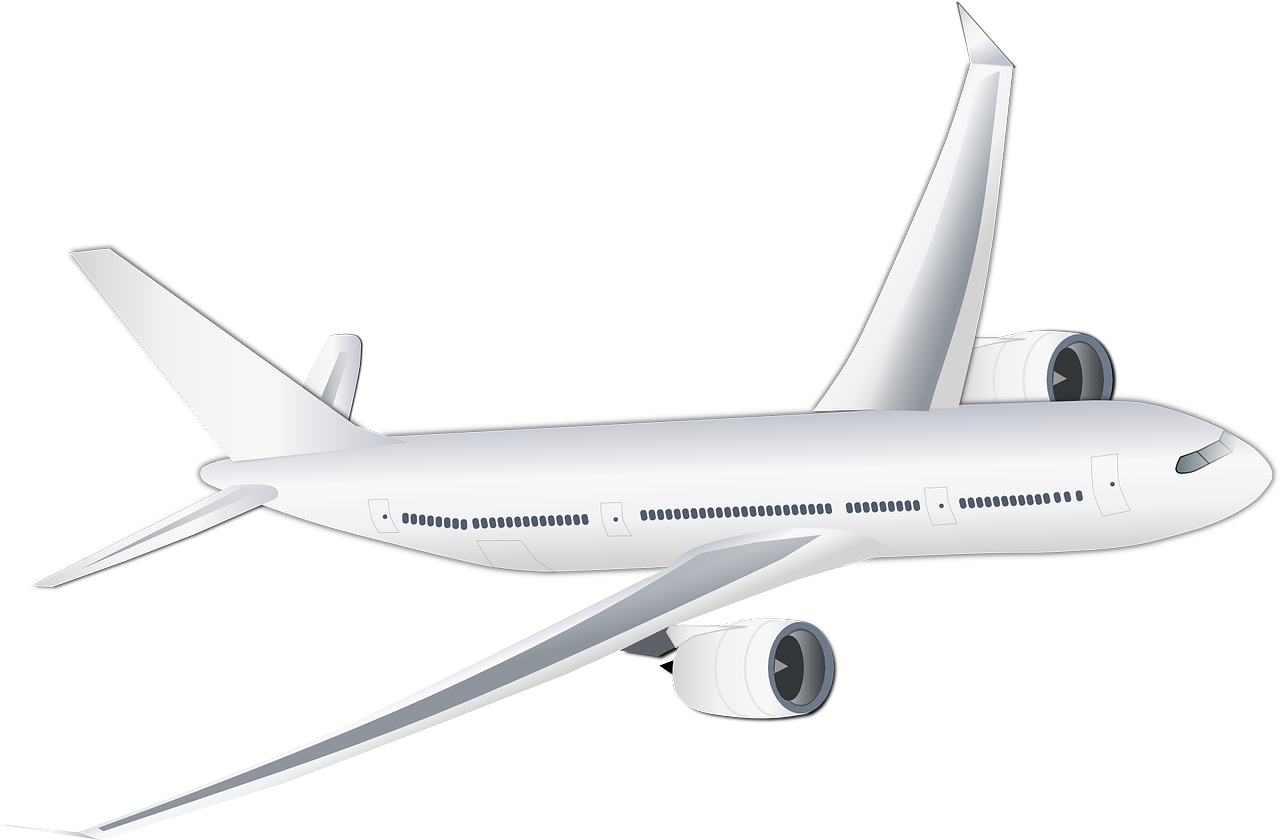
\includegraphics[width=\textwidth]{img/airplane.png}}; \\
\node(s2){
\includegraphics[width=\textwidth]{img/woman.png}};       \& \& \& \node(c2) {
\includegraphics[width=2\textwidth]{img/logistics.png}}; \\
\node(s3){
\includegraphics[width=\textwidth]{img/man.png}};         \& \& \& \node(c3) {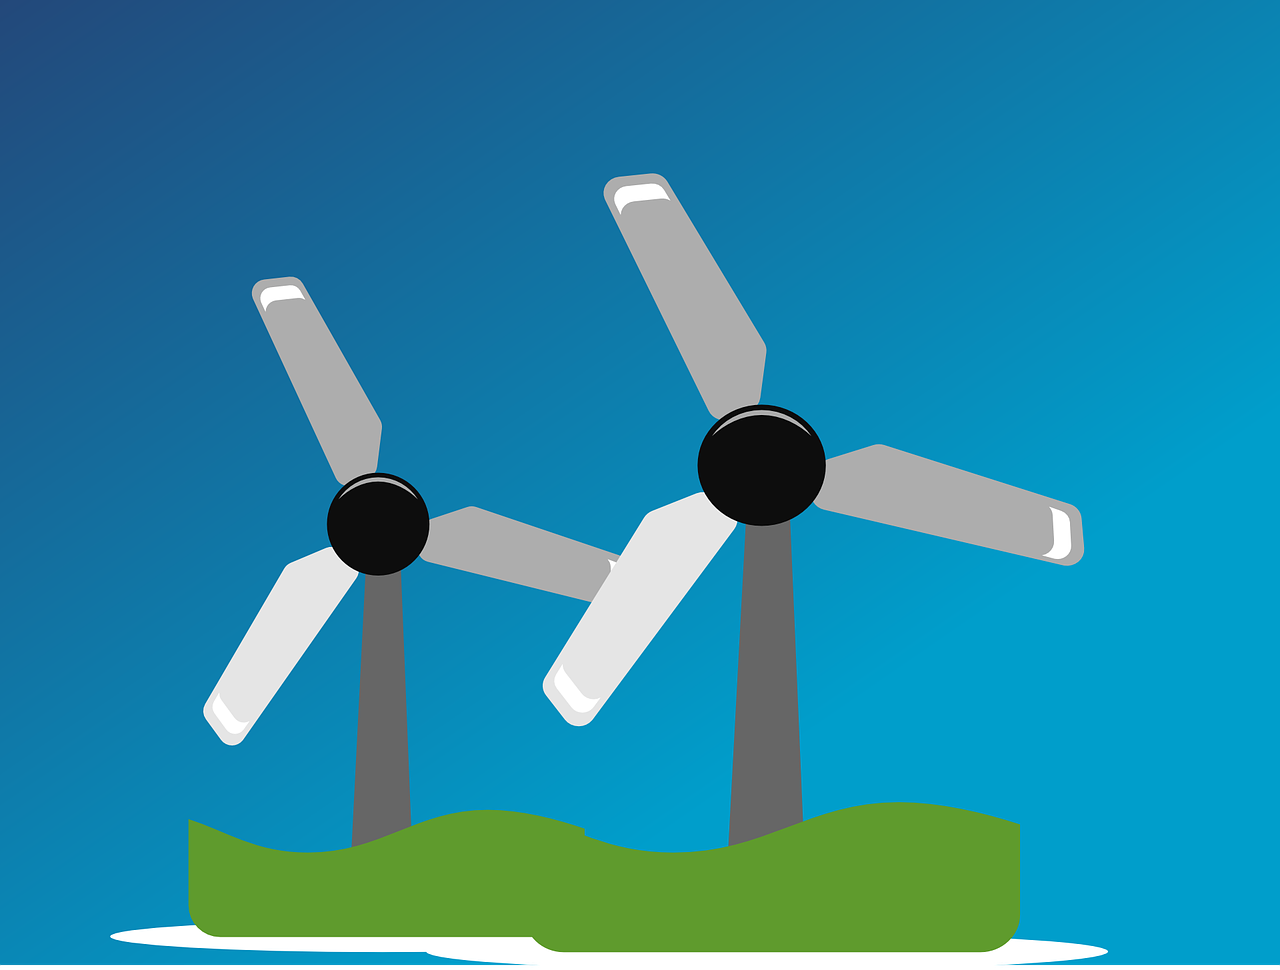
\includegraphics[width=2\textwidth]{img/enrgy.png}}; \\
\node[defaultStyle, draw, onslide={<3->{highlight2}}](s4){
\includegraphics[width=\textwidth]{img/woman2.png}};      \& \\
};

\draw[onslide={<2->{highlight}}] (s1) -- (c1);
\draw[] (s1) -- (c2);

\draw[onslide={<2->{highlight}}] (s2) -- (c1);
\draw[] (s2) -- (c3);

\draw[onslide={<2->{highlight}}] (s3) -- (c2);

\draw[onslide={<2->{highlight}}] (s4) -- (c3);
\draw[] (s4) -- (c2);
%
%\draw[onslide={<1-2>{highlight}}] (z) -- (3);
%\draw[onslide={<3>{highlight}}] (z) -- (2);
%
%\draw[onslide={<1-2>{highlight}}] (t) -- (2);
%\draw[] (t) -- (1);
%\draw[onslide={<3>{highlight}}] (t) -- (5);
%\draw[] (t) -- (3);
%\draw[] (t) -- (4);
%\draw[onslide={<1>{highlight}}] (u) -- (4);
%\draw[] (u) -- (3);
%\draw[] (u) -- (5);
%\draw[] (u) -- (6);
\end{tikzpicture}
\end{center}
\onslide<2->{Diese \alert{Zuweisung} respektiert die studentischen Präferenzen  (Kanten) \onslide<3->{ignoriert aber die  {\color{CornflowerBlue} Firmenpräferenzen}.}}
\onslide<4->{\tiny OK, es ist nicht wirklich ein \emph{Matching} da Firmen mehr als einen Studenten betreuen \ldots }
\end{frame}

\begin{frame}[fragile]{Mentor Matching: Constraint-Modell}
\begin{lstlisting}
int: n; set of int: STUDENT = 1..n;
int: m; set of int: COMPANY = 1..m;

% assign students to companies
array[STUDENT] of var COMPANY: worksAt;


int: minPerCompany = 1; int: maxPerCompany = 3;
constraint global_cardinality_low_up ( 
           worksAt, [c | c in COMPANY], 
           [minPerCompany | c in COMPANY], 
           [maxPerCompany | c in COMPANY]); 
           
solve 
search pvs_BAB();
\end{lstlisting}
\end{frame}

\begin{frame}[fragile]{Mentor Matching: FMSOFT Instanz}
\begin{lstlisting}
% fmsoft2016.mzn

n = 5; % students
m = 3; % companies

% student names for better readability 
int: raubholz = 1;
int: schraubale = 2;
int: meerfluss = 3; 
int: gleich = 4; 
int: lustig = 5; 

% company names 
int: delphi = 1;
int: cupgainini = 2;
int: youthlab = 3;

\end{lstlisting}

\end{frame}

\begin{frame}[fragile]{Mentor Matching: Präferenzen}
\begin{lstlisting}
PVS: students = new ConstraintRelationships("students") {
   soft-constraint raubholzdelphi: 'worksAt[raubholz] = delphi';
   soft-constraint raubholzyouthlab: 'worksAt[raubholz] = youthlab';
   soft-constraint gleichcupg: 'worksAt[gleich] = cupgainini';
   
   crEdges : '[| mbr.raubholzyouthlab, mbr.raubholzdelphi | 
                 mbr.gleichcupg, mbr.raubholzdelphi |]';
   useSPD: 'true' ;
}; 

PVS: companies = new ConstraintRelationships("companies") {
   soft-constraint delphi_meer: 'worksAt[meerfluss] = delphi';
   soft-constraint delphi_gleich: 'worksAt[gleich] = delphi';
   soft-constraint youthlab: 'worksAt[lustig] = youthlab';
   
   crEdges : '[| mbr.delphi_meer, mbr.delphi_gleich |]';
   useSPD: 'true' ;
}; 

\end{lstlisting}
\end{frame}

\begin{frame}[fragile]{Mentor Matching: Verhalten I}
\begin{lstlisting}
solve ToWeighted(students) lex ToWeighted(companies);
\end{lstlisting}
\begin{Verbatim}[fontsize=\small]
Intermediate solution:worksAt = [3, 2, 1, 1, 1]
Valuations: pen_companies = 1; pen_students = 3
----------
Intermediate solution:worksAt = [1, 2, 3, 1, 1]
Valuations: pen_companies = 2; pen_students = 2
----------
Intermediate solution:worksAt = [1, 3, 1, 2, 1]
Valuations: pen_companies = 3; pen_students = 1
----------
Intermediate solution:worksAt = [1, 1, 1, 2, 3]
Valuations: pen_companies = 2; pen_students = 1
----------
==========
\end{Verbatim}

\end{frame}

\begin{frame}[fragile]{Mentor Matching: Verhalten II}
\begin{lstlisting}
solve ToWeighted(companies) lex ToWeighted(students);
\end{lstlisting}
\begin{Verbatim}[fontsize=\small]
Intermediate solution:worksAt = [3, 2, 1, 1, 1]
Valuations: pen_companies = 1; pen_students = 3
----------
Intermediate solution:worksAt = [2, 1, 1, 1, 3]
Valuations: pen_companies = 0; pen_students = 4
----------
Intermediate solution:worksAt = [1, 2, 1, 1, 3]
Valuations: pen_companies = 0; pen_students = 2
----------
==========
\end{Verbatim}

\end{frame}


\begin{frame}[fragile]{Mentor Matching: WS 15/16}
\begin{itemize}
\item Präferenzen aus E-Mails vom WS 15/16 gesammelt

\begin{parchment}
\begin{verbatim}
"the favorites":
1. JuneDied-Lynx- HumanIT
2. Cupgainini
 
"I could live with that":
3. Seamless-German
4. gsm systems
5. Yiehlke
 
"I think, we won't be happy":
6. APS
7. Delphi Databases
\end{verbatim} 
\end{parchment}
\end{itemize}
\end{frame}

\begin{frame}[fragile]{Mentor Matching: WS 15/16}
\begin{itemize}
\item Priorität zu \alert{Studenten}
\begin{itemize}
\item[-] Was sollen Firmen schon mit unzufriedenen Mentees anfangen?
\end{itemize}
\item Suchraum: 7 Firmen für 16 Studenten $\rightarrow 7^{16} = 3.3233 \cdot 10^{13}$
\vspace*{2ex}
\item Führte zu einem Constraint-Problem mit
\begin{itemize}
\item[-] 77 student. Präferenzen (Soft Constraints) von 16 Studenten
\item[-] insgesamt 114 Soft Constraints (37 Firmenpräferenzen) 
\end{itemize}

\vspace*{2ex}

\item \emph{Bewiesen} optimale Lösung
\begin{itemize}
\item[-] 6 Minuten Lösungszeit
\end{itemize}
\end{itemize}
\end{frame}



\begin{frame}[fragile]{Prüfungstermine}

\textbf{Ziel}: Weise Prüfungstermine an Studenten zu, sodass
\begin{itemize}
\item Jeder Student stimmt seinem Termin zu 
\item Die Anzahl verschiedener Termine wird minimiert (um das Zeitinvestment der Dozenten zu schonen)
\end{itemize}

%\vspace*{2ex}
%\begin{parchment}
\begin{center}
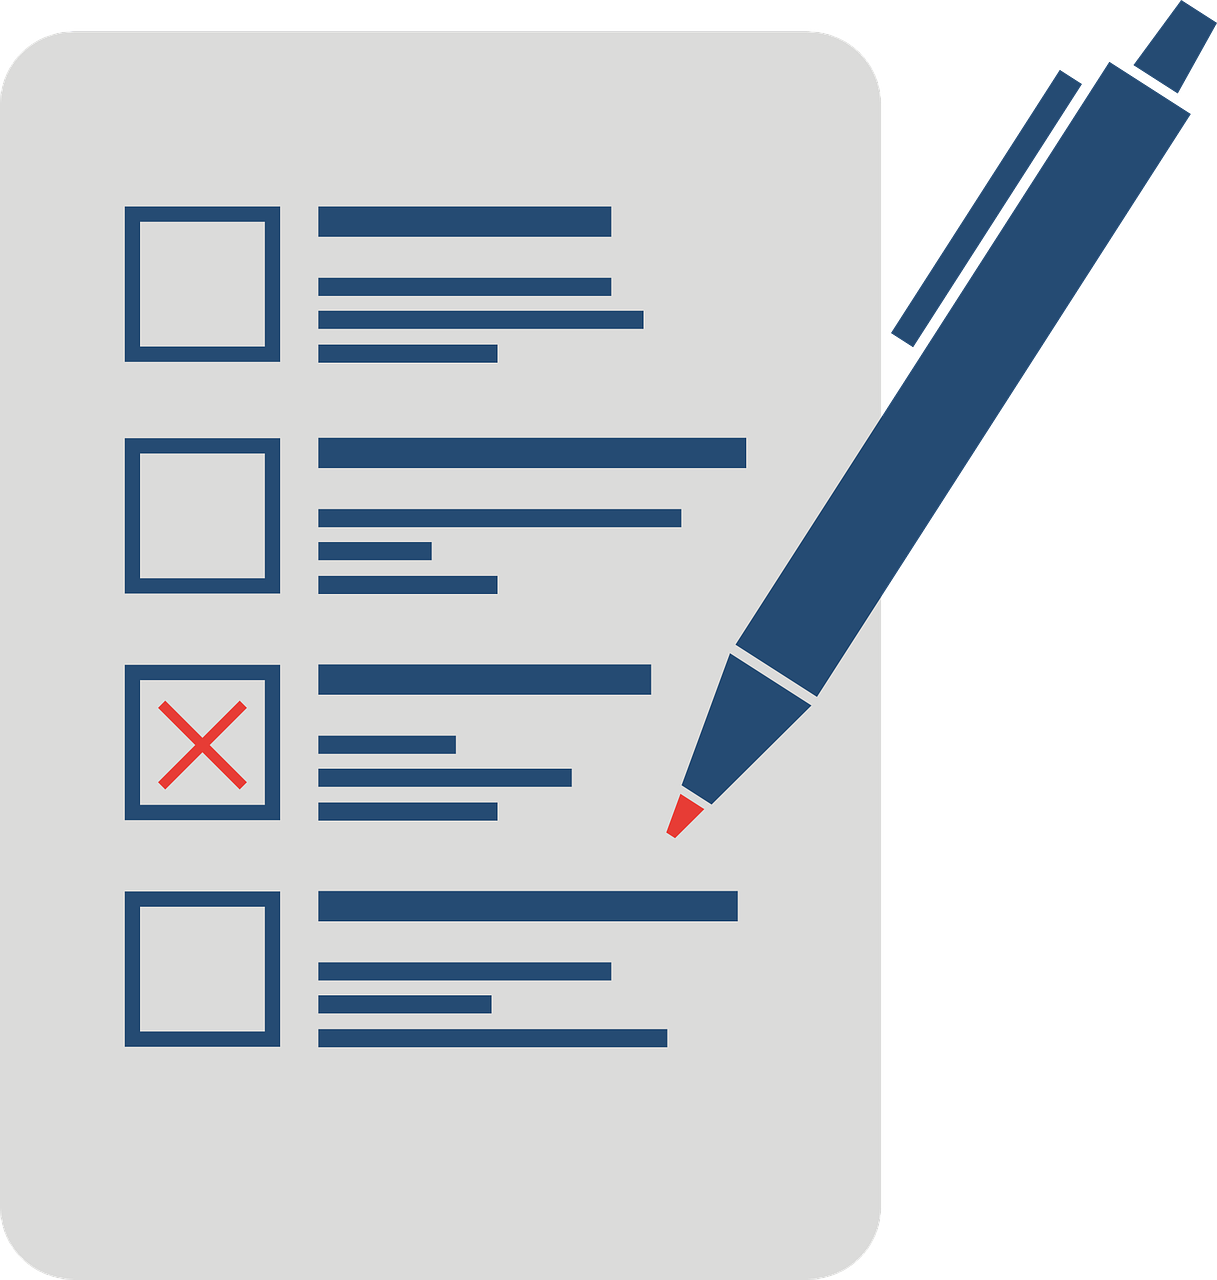
\includegraphics[width=.15\textwidth]{img/voting.png}
\hspace*{4ex}
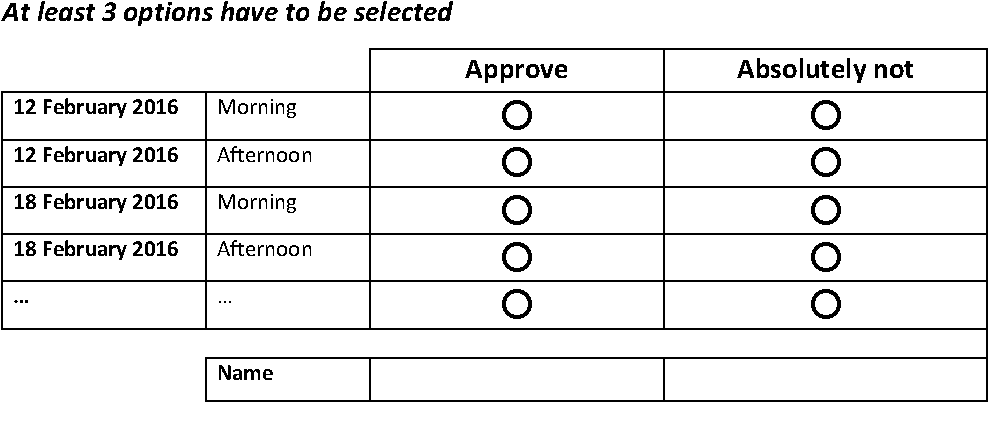
\includegraphics[width=.5\textwidth]{img/Voting.pdf}
\end{center}
%\end{parchment}

\begin{itemize}
\item Kein studentischer Wunsch sollte höher gewichtet werden
\item Prüfungsplan ist eine gemeinsame Entscheidung

\end{itemize}
\end{frame}

\begin{frame}[fragile]{Prüfungstermine: Constraint-Modell}
\begin{lstlisting}
% Exam scheduling example with just a set of 
% approved dates and *impossible* ones
include "globals.mzn";
include "soft_constraints/soft_constraints.mzn";

int: n; set of int: STUDENT = 1..n; 
int: m; set of int: DATE = 1..m;
array[STUDENT] of set of DATE: possibles;
array[STUDENT] of set of DATE: impossibles;

% the actual decisions
array[STUDENT] of var DATE: sd;

int: minPerSlot = 0; int: maxPerSlot = 4;
constraint global_cardinality_low_up(sd % minPerSlot, maxPerSlot
constraint forall(s in STUDENT) (not (sd[s] in impossibles[s])); 
 
\end{lstlisting}
\end{frame}

\begin{frame}[fragile]{Prüfungstermine: Präferenzen}

\begin{lstlisting}
include "../defs.mbr";
PVS: students = new WeightedCsp("students") {
   k: '100';
   soft-constraint raubholz:   'sd[raubholz] in {monday, tuesday}';   
   soft-constraint schraubale: 'sd[schraubale] in {tuesday, wednesday}';
   soft-constraint meerfluss:  'sd[meerfluss] in {tuesday}';
   soft-constraint gleich:   'sd[gleich] in {monday, tuesday}';
   soft-constraint lustig:     'sd[lustig] in {monday, wednesday}';
   % hard by weight (less than bottom)
   soft-constraint lustig-urlaub: 'sd[lustig] != tuesday'
                                :: weights('101'); 
}; 
PVS: teachers = new CostFunctionNetwork("teachers") {
   soft-constraint scheduledDates: 'scheduledDates';
}; 
solve students lex teachers;
\end{lstlisting}
\begin{Verbatim}[fontsize=\small]
Scheduled: [1, 2, 2, 1, 1], Distinct dates: 2
Valuations: mbr_overall_students = 0; mbr_overall_teachers = 2
\end{Verbatim}
\end{frame}


\begin{frame}[fragile]{Prüfungstermine: WS 15/16}

\begin{itemize}
\item Gesammelte Präferenzen von 33 Studenten
\item 12 mögliche Termine (6 Tage, Vormittag und Nachmittag)
\begin{itemize}
\item[-] \emph{Approval}-Menge 
\item[-] \emph{Impossible}-Menge
\end{itemize}

\vspace*{2ex}

\item Aggregiert via Wahl durch Zustimming (\alert{Approval voting}), hat ansprechende wahltheoretische Eigenschaften (Arrow)!
\item Höchstens 4 pro Termin

\item Sofort (61 msec) wurde eine optimale Lösung gefunden, die
\begin{itemize}
\item[-] von \emph{jedem} Student Zustimmung erhält
\item[-] Mit der Minimalanzahl von 9 Terminen auskommt
\end{itemize}
\item Verwendete Strategie (natürlich, \ldots):
\end{itemize}
\begin{lstlisting}
solve students lex teachers;% pro students
\end{lstlisting}
\end{frame}

\begin{frame}[fragile]{Energiefallstudie: Unit Commitment}

\textbf{Ziel}: Weise Kraftwerken Produktion zu, sodass
\begin{itemize}
\item Der Bedarf gedeckt wird
\item Steuerungsvorlieben (ökonomische Leistungsbereiche, \ldots) eingehalten werden
\end{itemize}
\fontsize{8pt}{7.2}\selectfont
\tikzset{
   main node/.style={rectangle,
                     rounded corners,
   					 fill=black!15,
   					 draw,
   					 minimum width=3.5em,
   					 text centered,
                     inner sep=2.5pt,	 
   					 font=\sffamily
   					},
   treestyle/.style={rectangle,fill=black!15,draw,font=\sffamily},
   constraint/.style={circle,fill=black!15,draw,font=\sffamily\small},
   constraint_satisfied/.style = {constraint, fill=white},
   constraint_violated/.style = {constraint, fill=black!25},
}

\begin{figure}[t]
\centering
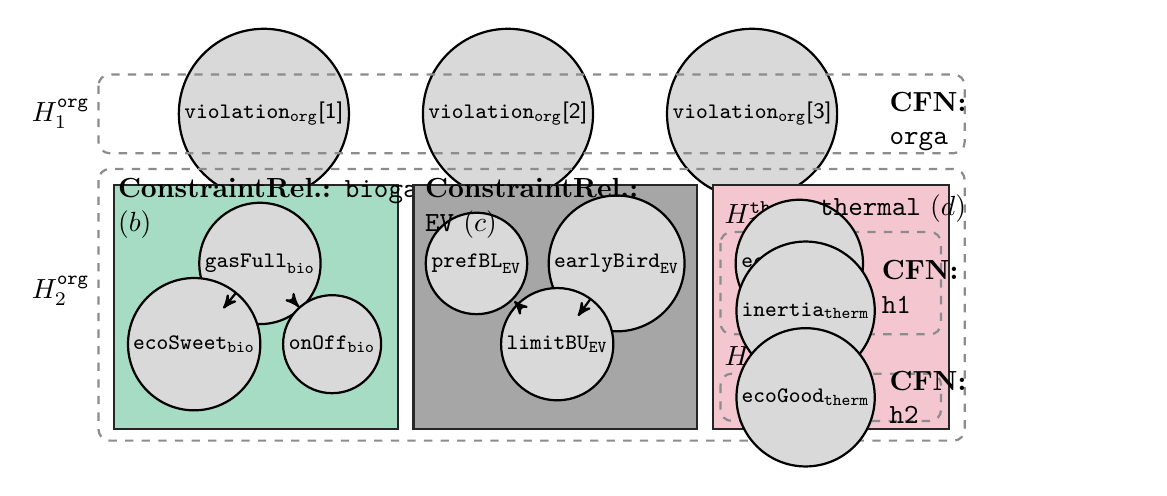
\begin{tikzpicture}[->,>=stealth',shorten >=1pt,auto,node distance=1.45cm,inner sep=1.5pt,outer sep = 0.0pt, thick] 
%\tikzstyle{every node}=[font=\tiny]
\begin{scope}[xshift=-6.0cm,yshift=-4.0cm]
\node[main node, style={font=\sffamily\footnotesize}] at (0.1,1.5) {\minMaxViolation[1]};
\node[main node, style={font=\sffamily\footnotesize}] at (3.2,1.5) {\minMaxViolation[2]};
\node[main node, style={font=\sffamily\footnotesize}] at (6.3,1.5) {\minMaxViolation[3]};

\draw [rounded corners,dashed,black!45] (-2,2) rectangle (9.0,1);
\node[text width=3cm, anchor=west, right] at (-2.9, 1.5) { \hLevelOrg{1} };
\draw [rounded corners,dashed,black!45] (-2,0.8) rectangle (9.0,-2.65);
\node[text width=4cm, anchor=west, right] at (-2.9, -0.75) { \hLevelOrg{2} };

% bio
\draw [black!85,fill=forestgreen!35] (-1.8,0.6) rectangle (1.8,-2.5);
\node[main node, style={font=\sffamily\footnotesize}] (5) at (0.05,-0.4) {\gasFull};
\node[main node, style={font=\sffamily\footnotesize}] (6) [below left of=5,xshift=5.4] {\ecoSweet};
\node[main node, style={font=\sffamily\footnotesize}] (7) [below right of=5,xshift=-3.1] {\onOff};
%\node[main node, style={font=\sffamily\footnotesize},double] (hardConstraint) [below left of=7,xshift=-3.1,yshift=7] {$\mathsf{maxProd}$};
\node[text width=4cm, anchor=west, left] at (2.3, 0.3) { \textbf{ConstraintRel.:}  $\mathtt{\biogas}$ $(b)$ };
%\node[text width=2cm, anchor=west, left] at (0.4, 0.3) { CR \textsc{TPD} };

% EV
\draw [black!85,fill=black!35] (2.0,0.6) rectangle (5.6,-2.5);
\node[main node, style={font=\sffamily\footnotesize}] (3) at (2.80,-0.4) {\prefBatteryLevel};
\node[main node, style={font=\sffamily\footnotesize}] (4) at (4.58,-0.4)  {\earlyBird};
\node[main node, style={font=\sffamily\footnotesize}] (8) [below right of=3] {\limitBatteryUsage};
\node[text width=3cm, anchor=west, left] at (5.2, 0.3) { \textbf{ConstraintRel.:}  $\mathtt{\ev}$ $(c)$ };
%\node[text width=2cm, anchor=west, left] at (4.3, 0.3) { CR };
%\node[text width=1cm, anchor=east, left] at (5.3, -2.3) { \textsc{SPD} };

% thermal
\draw [black!85,fill=thermicred!25] (5.8,0.6) rectangle (8.8,-2.5);
\draw [rounded corners,dashed,black!45] (5.9,0) rectangle (8.7,-1.3);
\node[text width=4cm, anchor=west, right] at (5.9, 0.2) { \hLevelThermal{1} };
\draw [rounded corners,dashed,black!45] (5.9,-1.8) rectangle (8.7,-2.4);
\node[text width=4cm, anchor=west, right] at (5.9, -1.6) { \hLevelThermal{2} };
\node[main node, style={font=\ttfamily\footnotesize}] (10) at (6.9,-0.4) {\ecoOpt};
\node[main node, node distance=0.85cm, style={font=\sffamily\footnotesize}] (11) at (6.98,-1.0) {\inertia};
\node[main node, node distance=0.85cm, style={font=\sffamily\footnotesize}] (12) at (6.98,-2.1) {\ecoGood};
\node[text width=4cm, anchor=west, right] at (7.1, 0.3) { $\mathtt{\thermal}$ $(d)$ };

\node[text width=2cm, anchor=west, left] at (10, -0.7) { \textbf{CFN:} \\ $\mathtt{h1}$ };

\node[text width=2cm, anchor=west, left] at (10.1, -2.1) { \textbf{CFN:} \\ $\mathtt{h2}$ };

\node[text width=2cm, anchor=west, left] at (10.1, 1.4) { \textbf{CFN:} \\ $\mathtt{orga}$ };

\path[every node/.style={font=\sffamily\tiny}]
  (8) edge node [right] {} (3)
  (8) edge node [right] {} (4)
  (6) edge node [right] {} (5)
  (7) edge node [right] {} (5)
;
\end{scope}

% \begin{scope}[xshift=-0.2cm,yshift=-0.9cm]
% \node[text width=9cm,left] at (0.0, 0.0) {%
% \begin{itemize}[itemsep=2pt]
%   \item something interesting
% \end{itemize}
% };
% \end{scope}

\end{tikzpicture}
%\caption{Case study depicting individual and organizational preference specifications in context.}
\label{fig:preferencesCaseStudy}
\end{figure}
  



%%% Local Variables:
%%% mode: LaTeX
%%% mode: TeX-PDF
%%% mode: TeX-source-correlate
%%% TeX-master: "../quality-quantity-soft-constraints.tex"
%%% End:


\end{frame}


\begin{frame}[fragile]{Unit Commitment: Constraint-Modell}
\begin{lstlisting}
int: T = 5; set of int: WINDOW = 1..T;
array[WINDOW] of int: demand = [20, 21, 25, 30, 29];

int: P = 3; set of int: PLANTS = 1..P;

array[PLANTS] of int: pMin  = [12, 5, 7];
array[PLANTS] of int: pMax  = [15, 11, 9];

array[WINDOW, PLANTS] of var 0..15: supply; 
constraint forall(p in PLANTS, w in WINDOW) 
     (supply[w,p] in pMin[p]..pMax[p]);

array[WINDOW] of var int: violation = 
    [ abs( sum(p in PLANTS) (supply[w, p]) - demand[w] ) | w in WINDOW];

solve search pvs_BAB();
\end{lstlisting}
\end{frame}

\begin{frame}[fragile]{Prüfungstermine: Präferenzen I}

\begin{lstlisting}
PVS: orga = new CostFunctionNetwork("Orga") {
    soft-constraint vio_1: 'violation[1]';
    soft-constraint vio_2: 'violation[2]';
    soft-constraint vio_3: 'violation[3]';
    isWorstCase: 'true';
};
PVS: biogas = new ConstraintRelationships("biogas") {
   soft-constraint gasFull: 
     'forall(w in WINDOW) (supply[w,biogas] >= 13)';
   soft-constraint ecoSweet: 
     'forall(w in WINDOW) (supply[w,biogas] >= 14)';
   soft-constraint onOff: 
     'forall(w in 1..T-1) ( 
        abs(supply[w,biogas] - supply[w+1,biogas]) <= 1)';
   
   crEdges : '[| mbr.ecoSweet, mbr.gasFull | mbr.onOff, mbr.gasFull |]';
   useSPD: 'true' ;
}; 
\end{lstlisting}
\end{frame}

\begin{frame}[fragile]{Prüfungstermine: Präferenzen II} \small

\begin{lstlisting}
PVS: ev = new ConstraintRelationships("ev") {...}; 

PVS: therm1 = new CostFunctionNetwork("therm1") {
  soft-constraint ecoOpt: 
    'sum(w in WINDOW) ( abs(supply[w,thermal] - 8) )';
  soft-constraint inertia: 
    'sum(w in 1..T-1) ( abs(supply[w,thermal] - supply[w+1,thermal]))';
};

PVS: therm2 = new CostFunctionNetwork("therm2") {
  soft-constraint ecoGood: 
    'sum(w in WINDOW) ( abs(supply[w,3] - 9) )';
};

solve orga lex ( biogas pareto ev pareto  (therm1 lex therm2) );
\end{lstlisting}
$P_{\mathtt{org}_1} \ltimes (P_{\prosumer{\biogas}} \times P_{\prosumer{\ev}} \times (P_{\prosumer{\thermal}}^1 \ltimes P_{\prosumer{\thermal}}^2))$
\end{frame}


\begin{frame}{Evaluationsergebnisse}

\end{frame}

\begin{frame}{Kooperationen}
\begin{itemize}
\item[] \alert{Konzepte, Sprachdesign MiniBrass}
\begin{itemize}
\item[-] AS, Alexander Knapp, Gerrit Anders, Oliver Kosak
\end{itemize}
\item[] \alert{Anwendungen, Multiagenten-Einsatz}
\begin{itemize}
\item[-] Alexander Schubert (MSc-Thesis: Einsatz von Voting-Verfahren), Markus Tolls (MSc-Thesis: Formalisierung von Task-Allocation-Problemen)
\end{itemize}
\end{itemize}
\end{frame}

\begin{frame}{Outreach}
\begin{itemize}
\item Vortrag Helmholtz-Zentrum München
\item Vortrag FH Hagenberg
\item Tutorial @ SASO 2016
\end{itemize}
\end{frame}



\begin{frame}[allowframebreaks]
        \frametitle{References}
        \bibliographystyle{apalike}
        \bibliography{../common}
\end{frame}


\end{document}

